\begin{figure}[thb]
  \centering
  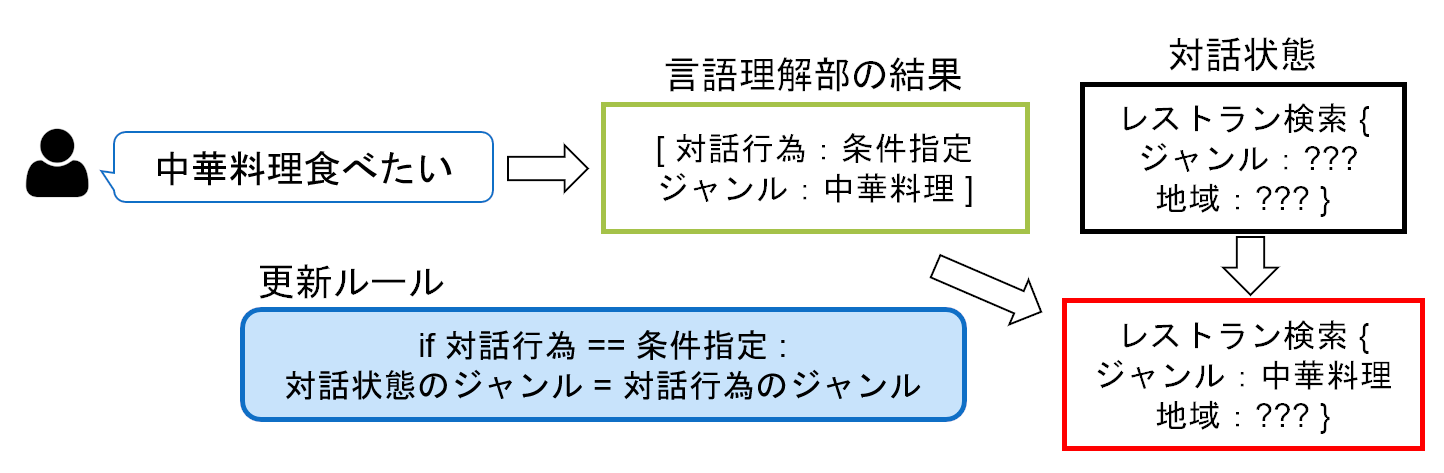
\includegraphics[width=15cm]{chapter2/rulebase.eps}
  \caption{if-then ルールによる対話状態追跡の例}
  \label{fig:rulebase}
\end{figure}

ルールベースの対話状態追跡とは,予め人間が決めた規則に従って対話状態を更新する対話状態追跡のことである.その規則は更新ルールと呼ばれ,プログラムやグラフによって定められる.
\par
一例として,if-then 文で記述されたプログラムを用いた対話状態追跡を図\ref{fig:rulebase}に示す.ルールベースの対話システムは図\ref{fig:rulebase}のように,言語理解部でユーザの対話行為も推定する.そして対話状態追跡は,言語理解部から得たユーザの対話行為によって条件分岐を行い,対話状態を更新していく.
\par
ルールベースの対話状態追跡は,後述する統計的機械学習や深層学習による対話状態追跡に比べて容易に行えるため,ほとんどの商用対話システムで採用されている.ただし,複雑な対話を扱うには多くの規則を定義する必要がある.また,言語理解部の結果に大きく依存するため,言語理解部で誤りが発生すると,自ずと間違った情報が対話状態に追加されるという問題がある\cite{rule_base}.